
\IEEEtitleabstractindextext{
\begin{abstract}
  Constructive solid geometry (CSG) is a widely used modeling tool. It constructs complex models by combining primitive solids with boolean operations. However, boolean evaluation, which computes the final model of CSG, has suffered from robustness problem for more than three decades. Some methods are fast but not robust, while some methods are robust but rely on exact arithmetic which is slow. Recent works tried to implement fast and robust boolean evaluation methods using plane-based representations (P-reps) of polyhedrons instead of vertex-based representations (V-reps) of polyhedrons. While they have achieved remarkable improvements, they are still slow compared with non-robust methods. We propose a fast and robust boolean method. It uses hybrid representations of polyhedrons, which combines P-reps with V-reps. The P-rep information is used for exact predicates computation and the V-rep information is used for coarse tests and fast topology query, which allows us to take advantages of both the efficiency of V-reps and the exactness of P-reps. Comparison experiments with the state-of-the-art show that our method is unconditionally robust for solid inputs, and is similarly efficient to existing non-robust methods.
\end{abstract}


\begin{IEEEkeywords}
boolean operations, CSG evaluation, plane-based geometry
\end{IEEEkeywords}

}

\maketitle


\IEEEdisplaynontitleabstractindextext
\IEEEpeerreviewmaketitle


\IEEEraisesectionheading{\section{Introduction}\label{sec:introduction}}
\IEEEPARstart{C}{onstructive} solid geometry (CSG) has long been a popular modeling tool for computer-aided design and computer-aided manufacturing (CAD / CAM). Complex models are constructed by combining primitives using regularized boolean operations \cite{requicha1977mathematical,tilove1980closure}: union, intersection, and difference. A CSG can be converted into the boundary representation (B-rep) through boolean evaluation. There are two major types of boolean evaluation methods, which vary according to how they deal with intersections between primitives.
Approximate methods \cite{wang2011approximate,pavic2010hybrid,biermann2001approximate} rediscretize the intersection areas, fit vertices approximatively, and rearrange the topology.
Conversely, exact methods \cite{ogayar2015deferred,douze2015quickcsg,zhou2016mesh} do not change vertex positions, and maintain as many input elements (such as faces, vertices, and topology) as possible. In many applications, exact methods are preferred for their accuracy. Additionally, the clear mapping between the surfaces of the input and output meshes in exact methods simplifies the inheritance of surface information, such as face colors and materials.

\begin{figure*}
  \centering
  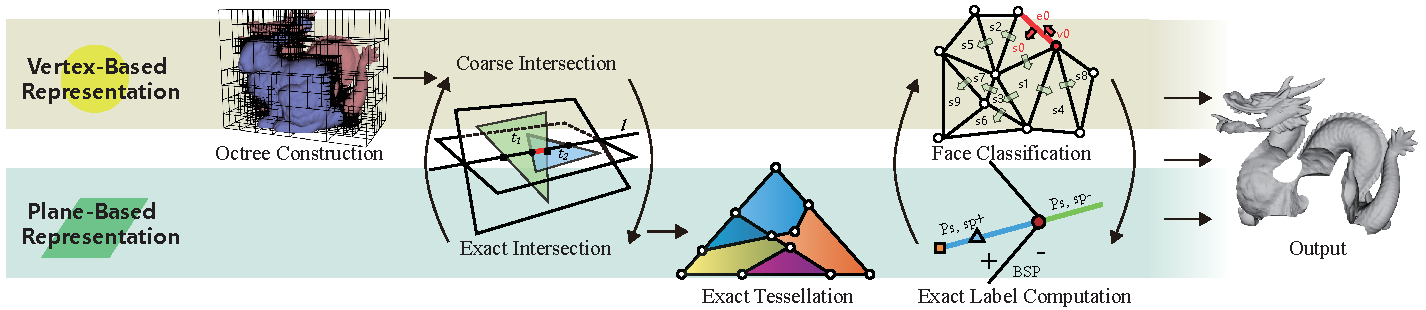
\includegraphics[width=7in]{overview}
  \caption{The illustration of our framework for boolean evaluation using hybrid representations. Vertex-based computation has its advantage of efficiency, and plane-based is necessary to guarantee exact geometry predicates. }\label{fig:hybrid}
\end{figure*}

However, there is always a compromise between robustness and efficiency for exact boolean algorithms.
Robust methods often require exact arithmetic \cite{barki2015exact,zhou2016mesh}, which is significantly slower than normal floating-point arithmetic.
Other methods only guarantee \textbf{quasi-robust} \cite{shewchuk1999lecture} by using unreliable techniques, such as epsilon-tweaking \cite{laidlaw1986constructive,feito2013fast,segal1990using} and numerical perturbation \cite{douze2015quickcsg}.
Recently, robust plane-based methods have been developed \cite{bernstein2009fast,campen2010exact} based on binary space partition (BSP) merging algorithms \cite{naylor1990merging,thibault1987set}.
The robustness of these methods is guaranteed by the theorem of Sugihara and Iri \cite{sugihara1990solid} that boolean evaluations can be performed without \textbf{constructions} \cite{shewchuk1999lecture} if polyhedrons are represented based on planes instead of vertices.
By only use \textbf{predicates}, boolean methods are easier to be robust.
These plane-based methods are generally faster than others which using exact arithmetic. However, they still suffer from performance issues because of the high computation complexity of BSP algorithms. In addition, the incoherence between BSP representations and B-reps of polyhedrons requires that extra steps for conversion and connectivity reconstruction, leading to worse performance.


Inspired by these previous studies, we develop a robust boolean method, which is unconditionally robust given consistent solid inputs, and is comparable efficient as non-robust methods. In our method, we combine P-reps with V-reps, forming hybrid representations of solids. Generally, the V-reps information is used for coarse tests and efficient neighboring face queries, while P-reps information is used for exact predicates (see Fig. \ref{fig:hybrid}). To avoid using exact arithmetic and ensure efficiency, we avoid constructions throughout our method.


Our method is different from the previous BSP-based methods \cite{bernstein2009fast,campen2010exact}.
While their methods are largely based on BSP theorem of \cite{naylor1990merging,thibault1987set}, our method is more like vertex-based methods such as \cite{feito2013fast,zhou2016mesh} and is significantly faster than these BSP-based methods. Our method is not a simple improvement of vertex-based methods, but a systematical solution for robustness of boolean evaluations. During intersection computation, we encode the triangle intersections into sets of planes, and then use these planes to determine exact tessellations. Subsequently, we classify each face in the tessellated meshes using small local BSP trees, which also compliment the P-reps to guarantee exactness. In order to guarantee performance, we try to minimize the usage of plane-based exact predicates in these stages. In addition, while most existing boolean methods can only process two meshes in each time, our method is \textbf{variadic} \cite{zhou2016mesh}, which can evaluate boolean expression with multiple input meshes immediately. Thus, our method reduce evaluation time of large CSGs by avoiding repetitive computation. Experiments have shown that our method is much faster than existing robust methods, and only around two times slower than non-robust methods.

\section{Related Work}


Boolean methods have been researched since their inception in the 1980s \cite{requicha1985boolean, laidlaw1986constructive}. Existing methods can be put into two categories: exact methods and approximate methods. Exact methods retain vertex positions, and the topology of the inputs is preserved as much as possible. The coordinates of intersection points between input meshes are computed by input configurations. However, the coordinates cannot be represented exactly using fixed-precision floating point numbers, hence exact arithmetic is needed for robustness. Conversely, approximate methods rediscretize the input mesh surfaces using techniques such as voxels, octrees, and Layered Depth Images (LDI). These methods generally have better performance and easier to be robust than exact methods, but the loss of precision and geometry information is inevitable. In this section, we first introduce previous work of these two categories, and then discuss plane-based boolean methods, which have close relation with our method.

\subsection{Exact Methods}


Some exact methods \cite{ogayar2015deferred,douze2015quickcsg,xu2013fast,feito2013fast,updegrove2016boolean}, are optimized for efficiency, but cannot guarantee robustness. They are implemented by fixed-precision floating-point arithmetic, so numerical errors are inevitable, which often leads to inconsistent results.
Douze et al. \cite{douze2015quickcsg} developed a very efficient method for handling very large meshes and arbitrary input primitives. However, this method makes general position assumption and cannot deal with coplanar situations.


On the other hand, some methods focus on robustness. The state-of-art method \cite{zhou2016mesh} try to handle a large range of topology deficiencies and guarantee to give solid outputs, with the cost of many extra computations such as self-intersecting test and vertex-rounding iterations.
As robustness problem results from numerical errors, many researchers have attempted use arbitrary precision arithmetic \cite{banerjee1996topologically, fortune1995polyhedral, keyser2004esolid, granados2003boolean, hachenberger2005boolean, zhou2016mesh,barki2015exact} and exact interval computation \cite{fang1993robustness, hu1996robust, segal1990using}. However, exact arithmetic are too expensive in terms of computation time. For example, CGAL's \cite{cgal:hk-bonp3-15a} exact-arithmetic implementation \cite{granados2003boolean} of Nef polyhedra \cite{bieri1988elementary} is more than 50 times slower than non-robust boolean operations \cite{bernstein2009fast}. Our method try to balance the performance and robustness, which guarantees the solid outputs under valid inputs without the use of exact arithmetic.


\subsection{Approximative Methods}


Because it is difficult to achieve efficiency, accuracy, and robustness simultaneously, some methods sacrifice accuracy for greater efficiency and robustness. Most such methods are based on volumetric representations of meshes. However, the quality of the resulting mesh depends on the resolution of the volume grid, and better quality requires significantly higher resolutions.
To accelerate this process, some methods reduce the complexity of the output mesh \cite{varadhan2004topology}, whereas others preserve non-intersected areas of the input mesh to avoid redundant tessellation \cite{pavic2010hybrid,wang2011approximate,zhao2011parallel,hable2005blister,ogayar2006gpu,updegrove2016boolean}.
Moreover, with the development of general-purpose computing on graphics processing units (GPGPU), many of them utilize the computational power of graphics hardware for boolean evaluations. These methods have good performance, and are suitable for interactive applications. However, the fundamental problem of approximate methods arises from the grid-dependent nature of volumetric calculations. They inevitably suffer from geometric detail loss and unwieldy topological changes.


\subsection{Plane-Based Methods}
\label{sec:pbrelated}

The concept of plane-based representations (P-reps) of polyhedrons was first described by Sugihara and Iri \cite{sugihara1990solid}. By using P-reps, boolean evaluations can be performed with only predicates, which are much easier to implement robustly. Berstein and Fussell \cite{bernstein2009fast} combined P-reps with BSP trees \cite{thibault1987set,naylor1990merging} to develop a boolean method which is unconditionally robust with consistent inputs. Unlike vertex-based methods, their method does not rely on exact arithmetic to be robust.
However, the merging of two BSP trees is has $O(mn)$ time complexity, where $m$ and $n$ are the size of the trees. Such high time complexity makes this method impractical for large meshes. Subsequently, Campen and Kobbelt \cite{campen2010exact} improved this method by localizing BSP operations using an octree. In this method, mesh refinements only take place locally near intersections, which leads to better performance. However, their method splits the intersection regions and non-intersection regions, and requires extra stitching step to reconstruct topology. Also, the performance of localized BSP merging is still poor compared with the vertex-based methods. Our method uses plane-based geometry to guarantee no error introduced during boolean evaluation, while reduces the performance impact from plane-based computation with V-reps information, which is much cheaper to use.
